\section*{Materials and Methods}

% model
We define an event as a conglomerate of information that encompasses
all of the social media content related to a real-world news
occurrence. Using this specification, which considers an event as a
complex unit of information, we measure the impact produced by an
event in terms of the strength or immediacy of the social network's
reaction to its information.  In particular, we measure an event's
impact using the \emph{arrival time intervals} between consecutive
social media messages in the event itself.
% The \emph{distribution} of the arrival time intervals is studied for
% a given event.
In those terms, we consider high-impact events to be those for which
the \emph{distribution} of arrival time intervals is most heavily
skewed towards the smallest possible interval, zero. In other words,
events for which most messages arrive in almost instant successions
are defined as high-impact.
%For example, Fig.~\ref{fig:example_buzz}
%shows the distribution of arrival time intervals for two events: {\em
%  (a) The death of Nelson Mandela} and {\em (b) The Oscars}. In this
%example,
For instance, we can observe that the majority of the messages about
the death of political leader Nelson Mandela
(Fig.~\ref{fig:nelson_mandela}) arrived within almost zero seconds of
each other. On the contrary, the messages about The Oscars
(Fig.~\ref{fig:oscars}) are much more spread out in time.
\begin{figure}
  \centering
  \begin{subfigure}{\textwidth}
    %\includegraphics[width=\textwidth]{figures/nelson_mandela_buzz_example}
    \caption{User posts about the death of Nelson Mandela arrive
      almost instantly.}
    \label{fig:nelson_mandela}
  \end{subfigure}%

  ~ %add desired spacing between images, e. g. ~, \quad, \qquad, \hfill etc.
  % (or a blank line to force the subfigure onto a new line)
  \begin{subfigure}{\textwidth}
    %\includegraphics[width=\textwidth]{figures/may_oscar_buzz_example}
    \caption{User posts about The Oscars arriving several weeks before
      the event.}
    \label{fig:oscars}
  \end{subfigure}%
  ~ %add desired spacing between images, e. g. ~, \quad, \qquad, \hfill etc.
  % (or a blank line to force the subfigure onto a new line)

  \caption{\textbf{Illustrative examples of two events
      summarized by our method. The event [nelson, mandela] (\ref{fig:nelson_mandela}) was
      collected on 2013-12-05. Since there is a high
      concentration in the first histogram bin, we conclude that the social media posts
      for this event occur in cascades of quick successions, almost
      instantaneously. The second event, [may, oscar] (\ref{fig:oscars}) was collected
      on 2014-03-23 discussing The Oscars event that was held a few
      weeks before. The arrival times of these posts are much more spread
      out. The $y$-axis is in square root scale.} 
  }
  \label{fig:example_buzz}
\end{figure}

%\newtext{ 
We introduce a novel vectorial representation called {\em
    impact-based event model}, which models an event's impact using
  its arrival time interval distribution.  This approach is inspired
  by the {\em codebook-based representation} from the field of
  multimedia content analysis, which is used, for example, in audio
  processing and computer vision~\cite{ff,Vaizman}.  In this model, a
  \emph{codebook} of the most common time intervals between
  consecutive messages on social media about a particular event is
  learnt from a large training corpus of events.  Subsequently, each
  event is represented as a histogram where the bins are the most
  representative time intervals.  The entries of the resulting vector
  are obtained as the percentage of consecutive message pairs of the
  event that are assigned to the corresponding bin, based on their
  arrival times.  In this representation it is important to note that
  event impact is relative to an event's overall size, and that the
  model is normalized with respect to the number of messages in the
  event. Hence, the only criteria considered while deciding whether or
  not an event is high impact is the portion of messages that were
  posted close in time to each other. This denotes the urgency
  assigned to the event by the social network independently of how
  many messages were posted overall.  %}

% Experimental analysis

We study a dataset of news events gathered from news
headlines from a \emph{manually curated} list of well-known news media
accounts (e.g., @CNN, @BreakingNews, @BBCNews, etc.) in the
microblogging platform Twitter \cite{Twitter_website}
%\footnote{\url{https://twitter.com}
%  (Accessed: August 25, 2015.)} 
(a full list of all the news media
accounts is provided in the supplementary material). Headlines were
collected periodically, every hour, over the course of approximately
one year. In parallel, all the Twitter messages (called \emph{tweets}) 
were extracted about each news event using the public
API \cite{Twitter_API}.
%\footnote{\url{https://dev.twitter.com/} (Accessed: August 25,
%  2015.)},
% In this research, since we focus on the microblogging platform
% Twitter, we collected all the Twitter messages (called
% \emph{tweets}) produced about each news event using the publicly
% available Twitter Search API
This process was performed by automatically extracting descriptive
sets of keywords for each event using a variation of frequent itemset
extraction \cite{Tan_Steinbach_Kumar} over the event's headlines.
These sets of keywords were then used to retrieve corresponding user
tweets for each event.  Overall, the dataset contains 43,256,261
tweets that account for 5,234 events (Table~\ref{table:dataset-stats}).

We illustrate an example of an event showing the set of keywords and a
sample of tweets associated with the event
(Fig.~\ref{fig:components}).  These keywords form a semantically
meaningful event; they refer to the incident where soccer player Luis
Suarez was charged for biting another player during the FIFA World Cup
in 2014. This general collection process results in a set of social
media posts associated to an event which can encompass several memes,
viral tweets and pieces of information. Therefore, the data about an
event can be considered more complex than that of existing studies
% \cite{Castillo:2014},\cite{Szabo:2010},\cite{Lerman:2010},\cite{Tatar:2011},\cite{Pinto:2013},\cite{Ahmed:2013,
% Zaman_information_spreading},\cite{suh2010want}
\cite{Castillo:2014,Szabo:2010,Lerman:2010,Tatar:2011,Pinto:2013,Ahmed:2013,suh2010want}
which typically focus on simpler pieces of information (e.g., one
particular meme, one viral tweet etc.).  We validate the events in our
data collection process to ensure that each group of social media
posts corresponds to a meaningful news event by calculating several
clustering metrics over its social media posts. We present a detailed
description of our collection methodology and how we construct
cohesive events in the supplementary material.

\begin{table}
  \centering
  \begin{tabularx}{\textwidth}{@{}p{6cm}llll@{}}
    \toprule
    \textbf{News events' property} & \textbf{Minimum} & \textbf{Mean} & \textbf{Median} & \textbf{Maximum} \\ \midrule
    \# of posts & 1,000 & 8,254 & 2,474 & 510,920 \\
    \# of keywords & 2 & 3.77 & 3 & 39 \\
    Event duration (hours) & 0.12 & 20.93 & 7.46 & 190.43 \\ \bottomrule
  \end{tabularx}
  \caption{\bf High-level description of the dataset of news events.} \label{table:dataset-stats}
\end{table}

\begin{figure}
  %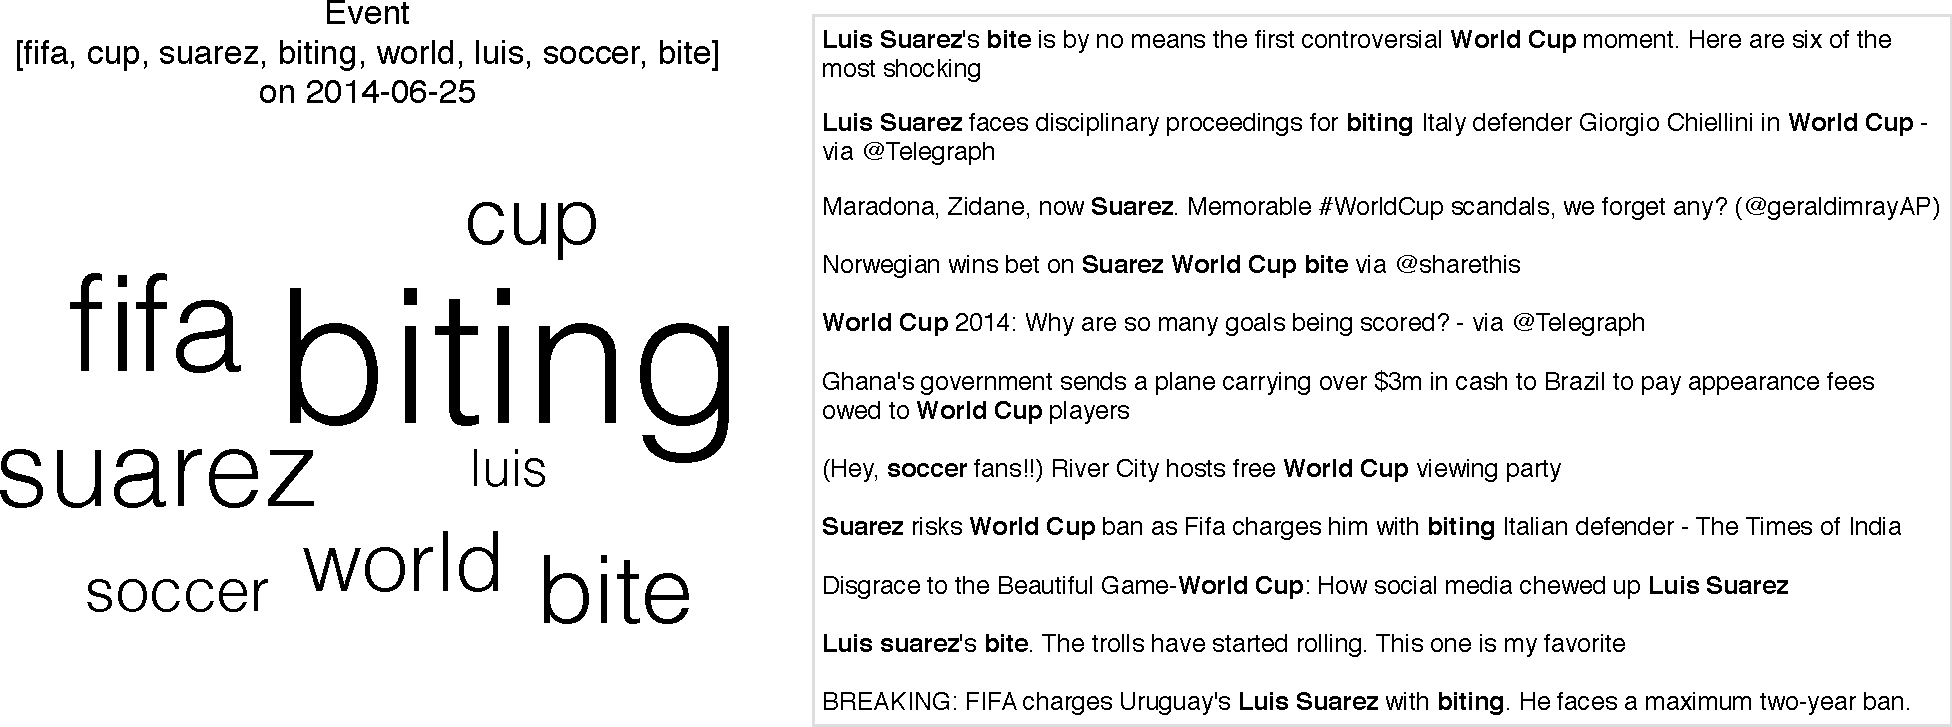
\includegraphics[width=\textwidth]{diagrams/suarez_example-crop}
  \caption{\textbf{A representative event, collected on 2014-06-25
      with keywords (left) and sample user posts (right) collected
      from the Twitter Search API. Collected user posts contain at
      least one pair of keywords. }}
  \label{fig:components}
\end{figure}


The collection of events is converted into their impact-based event
model representation. Using this model, we can identify events that
have produced similar levels of impact in the social network. In other
words, events are considered to have similar impact if the intervals
between their social media posts are similarly distributed, implying a
very much alike reaction to the events. In order to identify groups of
similar events, we perform clustering of the event models. We sort the
resulting groups of events from highest to lowest impact, according to
the concentration of social media posts in the bins that correspond to
short time intervals. We consider the events that fall in the top
cluster to be high-impact as their associated social media posts have
the shortest arrival time intervals.  In our dataset, these correspond
to roughly 8\% of the events.  We consider the next clusters in the
sorted ranking to form medium-high impact events, and so on.  Thus we
end with four groups of event histograms: high, medium-high,
medium-low and low (Fig.~\ref{fig:low_buzz_high_buzz}). This
classification of events based on their impact is independent of event
size. More details of this methodology is provided in the
supplementary material section titled `Event Model.'

\begin{figure}
  %\includegraphics[width=\textwidth]{figures/heatmap_summarized}
  \caption{\textbf{Each row is the average representation of all the
      events in that clusters.  A darker cell represents a higher
      value.  The y-axis specifies the number of events in that
      cluster.  Clusters are (top to bottom): high-impact, medium-high
      medium-low and low.}
    % \inote{Mauricio: change labels of x and y-axis (to: Event type
    % (total number of events))}
  }
  \label{fig:low_buzz_high_buzz}
\end{figure}